\documentclass[tikz,border=2pt]{standalone}
\usepackage{amsmath,amssymb}
\usepackage{pgfplots}
\pgfplotsset{compat=1.18}
\usetikzlibrary{arrows.meta}

\begin{document}
% Conditional variance: the spread of X around E[X | B] using the conditional pmf. Given
% B = {X >= 3} only the values 3 and 4 remain, so the spread shrinks from Var(X) = 1 to 12/49.
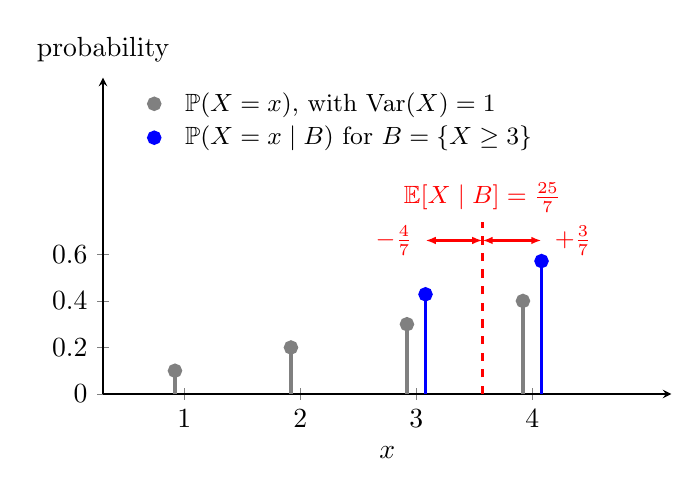
\begin{tikzpicture}
	\begin{axis}[
		axis lines=left, xmin=0.3, xmax=5.2, ymin=0, ymax=1.36,
		xtick={1,2,3,4}, ytick={0,0.2,0.4,0.6},
		xlabel={$x$}, ylabel={probability}, ylabel style={rotate=-90, anchor=south, at={(axis description cs:0,1.02)}},
		width=8.8cm, height=5.6cm, clip=false,
		legend style={draw=none, fill=none, font=\small, at={(0.03,0.99)}, anchor=north west}, legend cell align=left
		]
		\addplot[ycomb, gray, very thick, mark=*, mark size=2pt] coordinates {(0.92,0.1) (1.92,0.2) (2.92,0.3) (3.92,0.4)};
		\addlegendentry{$\mathbb{P}(X=x)$, with $\operatorname{Var}(X)=1$}
		\addplot[ycomb, blue, very thick, mark=*, mark size=2pt] coordinates {(3.08,0.4286) (4.08,0.5714)};
		\addlegendentry{$\mathbb{P}(X=x\mid B)$ for $B=\{X\ge3\}$}
		\draw[red, dashed, thick] (axis cs:3.571,0) -- (axis cs:3.571,0.74);
		\node[red, anchor=south, font=\small] at (axis cs:3.571,0.74) {$\mathbb{E}[X\mid B]=\tfrac{25}7$};
		\draw[{Latex[length=1.3mm]}-{Latex[length=1.3mm]}, red, thick] (axis cs:3.08,0.66) -- (axis cs:3.571,0.66);
		\draw[{Latex[length=1.3mm]}-{Latex[length=1.3mm]}, red, thick] (axis cs:3.571,0.66) -- (axis cs:4.08,0.66);
		\node[red, anchor=east, font=\small] at (axis cs:3.05,0.66) {$-\tfrac47$};
		\node[red, anchor=west, font=\small] at (axis cs:4.11,0.66) {$+\tfrac37$};
	\end{axis}
	
\end{tikzpicture}
\end{document}
